% +------------------------------------------------------------------------+
% | CGAL Reference Manual:  qt_widget.tex
% +------------------------------------------------------------------------+
% | Using Qt_widget to visualize CGAL Objects
% | 
% |
% |
% | 12.12.2001  Radu Ursu
% | 
\RCSdef{\qtwidgetRev}{$Revision$}
\RCSdefDate{\qtwidgetDate}{$Date$}
% +------------------------------------------------------------------------+

\newcommand{\qt}{{\em Qt}}      %QT abbreviation

\gdef\lciIfHtmlClassLinks{\lcFalse}
\gdef\lciIfHtmlRefLinks{\lcFalse}
\gdef\lciIfHtmlLinks{\lcFalse}

\chapter{Qt\_widget}
\label{chapterQtwidget}

\ccChapterRelease{\qtwidgetRev. \ \qtwidgetDate}\\
\ccChapterAuthor{Radu Ursu}


\begin{figure}[h]
\begin{ccTexOnly}
\begin{center}
\includegraphics{triangulation.eps} 
\end{center}
\end{ccTexOnly}
\begin{ccHtmlOnly}
<CENTER>
<IMG BORDER=0 SRC="triangulation.gif"  ALIGN=center  ALT="A Nice Screen Shoot">
</CENTER>
\end{ccHtmlOnly}
\end{figure}

\qt\ is a {\sc Gui} toolkit\footnote{http://www.trolltech.com} for
cross-platform application development. 

% +-----------------------------------------------------+
\section{Introduction}

In this chapter we describe a widget and some helper classes that
allow to interact with two dimensional \cgal\ objects in \qt\/ based applications.

The most important class is the class \ccStyle{Qt_widget}. It provides
a drawing area and output stream operators for \cgal\ objects, as well
as zooming and panning functionality.

The \ccStyle{Qt_widget} allows to attach {\em layers}. Layers usually
draw on the drawing area of the widget. Layers can be activated and
deactivated, and what you see in the drawing area is the overlay of
all attached activated layers. Layers can be used also for entering
input, and \cgal\ provides input \ccc{layers} for the two-dimensional
\cgal\ objects.

Finally, we provide a {\em toolbar} for controlling the basic functionality
of the \ccStyle{Qt_widget}.

The following sections describe the main class as well as the helper classes
in more detail and give examples that can be taken as starting points for
new applications.


\noindent {\bf Remark:} The \ccStyle{Qt_widget} is distributed under
the {\sc Qpl}, which is Trolltech's open source license. For more details
on the {\sc Qpl} see the file license.qpl in this \cgal\ distribution
or \verb+http://www.trolltech.com/developer/licensing/qpl.html+.

\section{Qt\_widget}
\label{Qt_widget}

The class \ccStyle{Qt_widget} is derived from the \qt\ class \ccStyle{QWidget}%
\footnote{A widget is the atom of the user interface: It receives mouse, keyboard and other 
events from the window system, and paints a representation of itself on the 
screen. Every widget is rectangular, and they are sorted in a Z-order. A 
widget is clipped by its parent and by the widgets in front of it.} 
which is the base class of all \qt\ user interface objects. 


The \ccStyle{Qt_widget} provides output operators for all \cgal\
objects. There are operators defined for output of : points, segments, 
lines, rays, circles, triangles, rectangles, polygons, conics,  and all type of
triangulations. Also some operators are defined to set
\ccStyle{Qt_widget}'s properties, like background and fill color, as
well as line width and point size.

As the following examples show, simple applications can be written
without the layers.

\subsection{Example: Hello Segment}
The first example draws a red segment on an orange background.
\ccIncludeExampleCode{Qt_widget/Examples/hellosegment.C}

Note that we call new but not delete. This does not mean that there is 
a memory leak. It is in Qt's responsability to free widgets.

We follow the \qt\ naming conventions for material properties, for
example, the {\tt CGAL::BackgroundColor} above.

All the drawing code should be put between \ccStyle{Qt\_Widget}'s lock() and
unlock() functions. See the manual reference pages of
\ccStyle{Qt\_widget}. Doing like this, the window will be updated only
once, when \ccStyle{Qt\_widget} finds the last unlock(). This way you
can avoid the window flickering.

This example has a severe drawback: When you resize the window it is
empty, as nothing is redrawn, that is this style of programs makes
only sense, if you quickly want to validate output of a geometric
computation. As in any event driven {\sc Gui} application, you have to provide 
a draw callback so that the window system can update the drawing
whenever necessary. This is the topic of the next example.

\subsection{Example: Draw Callback}

This example is slightly more involved. The user can enter points and
the application draws the Delaunay triangulation of the point set. 

\ccIncludeExampleCode{Qt_widget/basic/tutorial2/tutorial2.C}

As most {\sc Gui} toolkits Qt is event driven.  In the last line
of function \ccc{main}, the program enters an event dispatch loop.

When events, like keyboard or mouse events, happen, they
are forwarded to the widget that has focus.  Whenever one
presses a mouse button on the drawing area of the \ccc{CGAL::Qt\_widget},
the callback \ccc{mousePressEvent(QMouseEvent*e)} is called.
The event itself carries information about the position of the mouse.

In the example you see some \qt\ specific keywords that we explain
next.

Signals are declared by using the keyword \ccc{signals:} just like an
access specifier in your class declaration. When a component wants to
send out a \ccc{signal}, it uses the keyword \ccc{emit}. Slots are
declared and implemented just like any other \CC\ method. Slots can
have any parameters, but to be connected to a certain signal, they
must use the same parameter types as the signal. To use signals and
slots in your code, you must be able to bring them together. This is
done with the method \ccc{QObject::connect()}, which connects one
signal to one slot. This method needs to know four things: the object
that sends out the signal, the signal that it should connect the slot
to, the object that will receive the signal, and the slot that will be 
connected to the signal. The signal and slot are just typed in with
their names and parameter types, and wrapped with {\sc Signal()} and
{\sc Slot()}, respectively.

Every class that wants to define at least a single signal or slot must 
be derived from the class \ccc{QObject}. Every class definition that
wants to declare at least a single signal or slot must contain the
macro {\sc Q\_object}.

Whenever you define a class of your own that uses \ccc{signals} and/or
\ccc{slots}, it is not enough to simply compile it. You must also run
\ccc{moc}, the Meta-Object Compiler supplied with \qt\, on the file
the class declaration is in. Running \ccc{moc} outputs glue code that
is needed for the signal/slot mechanism to work. You have two
possibilities to add this glue code to your application: either you
include the code generated by \ccc{moc} in one of your source files or 
you compile the code generated by \ccc{moc} separately and link it to your
application.\footnote{See the \qt\ documentation related to signals/slots/moc.}

The line \ccc{//moc_source_file : tutorial2.C} is for users that use
makefiles. This line tells to the \cgal\ makefile generator that
\ccc{tutorial2.C} should be the file that \ccc{moc} should be run on
and include the code generated in this file. This is useful when you
have some header fies in different directories and you want that
\ccc{moc} parse them and include the code in the right files. If you
are not using makefiles you should not be concerned about this line.

The control flow in the example is now as follows. When you press the
mouse button, a point is inserted in the triangulation.  The widget's
method \ccc{redraw} is called. At the end it emits a signal, which is
connected to the slot of \ccc{My_window::redraw_win()}. In this
function the drawing if the Delaunay triangulation then finally
happens.  Note that the very same happens automatically when you
resize the window.

\section{Layers}
\label{Qt_widget_layers}
\subsection{Using Layers to Draw}

In the examples from the previous section the code for drawing on the
widget was in the \ccStyle{redraw_win()} function. As soon as the
applications are more involved it leads to a more modular design if
one delegates the drawing task to {\em layers}. For example, if the
application displays a Delaunay triangulation, the corresponding
Voronoi diagram, and at the same time highlights the nearest vertex to
the mouse coordinates, it makes sense to have three independent
layers. Besides better code, layers have the advantage that they can
be activated and deactivated at runtime. Finally, more modularity
means a higher potential for reuse.

A layer can be {\em attached} to a \ccc{Qt_widget}. The widget calls
the method \ccc{Qt_widget_layer::draw()} of all attached layers, in the
order that they were attached. It is a very simple rule: the last layer
attached will be drawn on top.

Also a layer can be {\em activated} and {\em deactivated}. Only active
layers are drawn, and by default a layer is activated when it gets
attached.  Note that deactivating and activating do not influence the
order of layers. You can change the order only by attaching and
detaching it.


\cgal\ provides a base class so that users can write their own
layers. All the layers derived from this base class
\ccc{Qt_widget_layer} have the functionality described.


\subsection{Example: Using a Layer to Draw}
\ccIncludeExampleCode{Qt_widget/basic/tutorial3/tutorial3.C}

This example defines a class derived from
\ccStyle{Qt_widget_layer}. In the member function \ccStyle{draw()}
is the code for drawing the triangulation. In \ccStyle{My_Window}
class you need an instance of \ccStyle{My_Layer} and you will 
have to attach it, if you want to see what the layer draws on the
screen.

As you see, this example is very similar to the previous one, but
the code for drawing the triangulation is no longer in the
\ccStyle{redraw_win()} function, but in a layer.



\subsection{Using Layers to Build New Objects }
\label{Qt_widget_tools}

The main purpose of layers is to have more modular code for drawing on
the widget. Things are similar for handling input. In the previous
examples, input went through the \ccc{Qt_widget::mousePressedEvent()}
callback, which interpreted the input. In applications where you have
different kinds of input, e.g., segments and polygons in an
arrangement demo, this quickly leads to unreadable, difficult to maintain
code,  especially as typically more than one event callback is
involved. The proper way of decomposition, is delegation
of the event handling to a {\em layer}. 

A layer for \ccStyle{Qt_widget} receives all the events from
\ccStyle{Qt_widget} if it is active and can provide some functionality
like input objects for \ccStyle{Qt_widget}. Notice that the layers
receive events in the order they have been attached. Layers can have
internal state, because for entering complex objects it needs several
events. Therefore layers must have functions to initialize state when
they are activated and to clean up when they are deactivated.

\cgal\ provides some predefined input layers. You can have a lot of
layers attached that could be active in the same time. You have to
take care how you manage the events if you do not want to have
conflicts. A conflict is when two attached layers that are active need 
both the same event and getting and using it might not have such a
good effect in your application. For example the predefined layers that 
builds a new line and a new circle produce bad visual effects when are 
both active.

You can resolve conflicts by using \ccc{layers} exclusive. If you have 
several layers that can not be active at the same time without creating
conflicts, you can resolve that by letting the user not activate
more than one of those at a time.

\begin{ccAdvanced}
In all the \cgal\ demos that are provided, the layers are used with a
toolbar and buttons. To activate and deactivate a layer you have to
click one of the toolbar buttons. There are layers that need exclusive 
use. This is accomplished by grouping the buttons in one group, and
making that group exclusive. The group class is \ccc{QButtonGroup} that
comes with \qt\ .
\end{ccAdvanced}

We first show how to use layers and then how they work.

\subsection{Example: How to Use a Layer}

In the previous section, you could insert new points in the
triangulation by clicking on the widget. This example shows how
the same can be achieved with the help of a layer.

We attach the predefined layer \ccc{Qt_widget_get_point} to the widget,
and connect the signal emitted by the widget to the function that
handles the input.  When the user clicks with the left mouse button,
the layer creates a point and passes it to the widget. The widget then
creates a signal that gets passed to the connected slot
\ccc{My_Window::get_new_object(CGAL::Object)}.

\ccIncludeExampleCode{Qt_widget/Examples/layer.C}

The \ccStyle{Qt_widget} forwards all events that it receives to the
attached and active layers. If a layer is attached but not active, it
does not get the events. It is put in a passive state. Activating and
deactivating the layer does not mean that the object is destructed,
you have to take care what should be the construction and destruction
code for your layers.

\subsection{Example: How Layers Work}

The following is an example of a \ccc{layer} that creates \cgal\ points when
the user clicks the left mouse button over the widget. 
 
\begin{ccExampleCode}
namespace CGAL {
template <class R>
class Qt_widget_get_point : public Qt_widget_layer
{
public:
  typedef typename R::Point_2   Point;
  typedef typename R::FT        FT;
  
  Qt_widget_get_point(const QCursor c=QCursor(Qt::crossCursor)) :
    cursor(c) {};
  
private:
  void mousePressEvent(QMouseEvent *e)
  {
    if(e->button() == Qt::LeftButton)
    {
      FT x=static_cast<FT>(widget->x_real(e->x()));
      FT y=static_cast<FT>(widget->y_real(e->y()));
      widget->new_object(make_object(Point(x, y)));
    }
  };
  void activating()
  {
    oldcursor = widget->cursor();
    widget->setCursor(cursor);
  };
  
  void deactivating()
  {
    widget->setCursor(oldcursor);
  };

  QCursor cursor;
}//endclass;
}//namespace CGAL
\end{ccExampleCode}

The \ccc{Qt_widget} forwards mouse and keyboard events to the attached tool.
In the above example only the \ccc{mousePressEvent} member function is overloaded.

Tools that create new \cgal\ objects, must call the member 
function \ccStyle{Qt_widget::new_object(CGAL::Object)}. The
\ccStyle{Qt_widget} then emits the signal
\ccStyle{new_cgal_object(CGAL::Object)}. This signal can be routed to
any slot of other object accepting a \ccc{CGAL::Object}, with the
following connect statement:
\begin{ccExampleCode}
connect(qt_widget_ptr, SIGNAL(new_cgal_object(CGAL::Object)), 
        any_other_object_ptr, SLOT(any_other_slot(CGAL::Object)));
\end{ccExampleCode}

The first argument must be a pointer to an instance of \ccc{Qt_widget}.
In the example we connect it to \ccc{MyWindow::get_new_object(CGAL::Object)}.

\section{The Standard Toolbar}
\label{Qt_widget_standard_toolbar}

The \ccStyle{Qt\_widget} allows to zoom and pan. This functionality is 
accessible through the class \ccStyle{Qt_widget_standard_toolbar}. The 
example further down shows how to use it in your application.

\begin{figure}[h]
\begin{ccTexOnly}
\begin{center}
\includegraphics{standard_toolbar.eps} 
\end{center}
\end{ccTexOnly}
\begin{ccHtmlOnly}
<CENTER>
<IMG BORDER=0 SRC="standard_toolbar.gif"  ALIGN=center  ALT="The
standard toolbar">
</CENTER>
\end{ccHtmlOnly}
\end{figure}

\newcounter{bean}
The functionality of the toolbar is like this from the left to right:
\begin{description}
%       {Button---\Roman{bean}}{\usecounter{bean}\setlength{\rightmargin}{\leftmargin}}
        \item[Point tool:] Deactivate the standard layers from the
standard toolbar.
	\item[History back:] Go back into the transformation history
	\item[History forth:] Go forth into the transformation history
        \item[Zoom In:] The scaling factor is multiplied by two
keeping the same center.
        \item[Zoom Out:] The scaling factor is divided by two keeping
the same center.
        \item[Focus on Point:] Lets you choose the center of the
region where you want to focus.
        \item[Focus on the Region:] The area in the rectangle that you selected will be magnified to best fit in the window.
        \item[Hand Tool:] Used for translate. Click to select the
first point of translation and drag to select the second point.
\end{description}

You can select a layer by clicking on a button of the standard
toolbar. To deactivate the layer you should press on the arrow button.

\ccExample
\ccIncludeExampleCode{Qt_widget/Examples/standard_toolbar.C}

This example generates 100 points and inserts them in a Delaunay
triangulation. Using the standard toolbar you can zoom in, zoom out,
translate.

\section{Some Predefined Icons}
\label{The predefined icons}

\cgal\ provides some icons defined in some header files. This icons are
pixmaps, having the extension \ccc{.xpm}. All the icons are enumerated right
here:

\ccInclude{CGAL/IO/pixmaps/arrow.xpm}
\begin{ccTexOnly}
\mbox{
\includegraphics{arrow_but.eps}}
\end{ccTexOnly}
\begin{figure}[h]
\begin{ccHtmlOnly}
<CENTER>
<IMG BORDER=0 SRC="arrow_but.gif"  ALIGN=center  ALT="">
</CENTER>
\end{ccHtmlOnly}
\end{figure}


\ccInclude{CGAL/IO/pixmaps/hand.xpm}
\begin{ccTexOnly}
\mbox{\includegraphics{hand_but.eps}}
\end{ccTexOnly}
\begin{figure}
\begin{ccHtmlOnly}
<CENTER>
<IMG BORDER=0 SRC="hand_but.gif"  ALIGN=center  ALT="">
</CENTER>
\end{ccHtmlOnly}
\end{figure}

\ccInclude{CGAL/IO/pixmaps/holddown.xpm}
\begin{ccTexOnly}
\mbox{\includegraphics{holddown_but.eps}}
\end{ccTexOnly}
\begin{figure}
\begin{ccHtmlOnly}
<CENTER>
<IMG BORDER=0 SRC="holddown_but.gif"  ALIGN=center  ALT="">
</CENTER>
\end{ccHtmlOnly}
\end{figure}

\ccInclude{CGAL/IO/pixmaps/mouse_coord.xpm}
\begin{ccTexOnly}
\mbox{\includegraphics{mouse_coord_but.eps}}
\end{ccTexOnly}
\begin{figure}
\begin{ccHtmlOnly}
<CENTER>
<IMG BORDER=0 SRC="mouse_coord_but.gif"  ALIGN=center  ALT="">
</CENTER>
\end{ccHtmlOnly}
\end{figure}

\ccInclude{CGAL/IO/pixmaps/point.xpm}
\begin{ccTexOnly}
\mbox{\includegraphics{point_but.eps}}
\end{ccTexOnly}
\begin{figure}
\begin{ccHtmlOnly}
<CENTER>
<IMG BORDER=0 SRC="point_but.gif"  ALIGN=center  ALT="">
</CENTER>
\end{ccHtmlOnly}
\end{figure}

\ccInclude{CGAL/IO/pixmaps/line.xpm}
\begin{ccTexOnly}
\mbox{
\includegraphics{line_but.eps}}
\end{ccTexOnly}
\begin{figure}
\begin{ccHtmlOnly}
<CENTER>
<IMG BORDER=0 SRC="line_but.gif"  ALIGN=center  ALT="">
</CENTER>
\end{ccHtmlOnly}
\end{figure}

\ccInclude{CGAL/IO/pixmaps/circle.xpm}
\begin{ccTexOnly}
\mbox{\includegraphics{circle_but.eps}}
\end{ccTexOnly}
\begin{figure}
\begin{ccHtmlOnly}
<CENTER>
<IMG BORDER=0 SRC="circle_but.gif"  ALIGN=center  ALT="">
</CENTER>
\end{ccHtmlOnly}
\end{figure}

\ccInclude{CGAL/IO/pixmaps/polygon.xpm}
\begin{ccTexOnly}
\mbox{\includegraphics{polygon_but.eps}}
\end{ccTexOnly}
\begin{figure}
\begin{ccHtmlOnly}
<CENTER>
<IMG BORDER=0 SRC="polygon_but.gif"  ALIGN=center  ALT="">
</CENTER>
\end{ccHtmlOnly}
\end{figure}

\ccInclude{CGAL/IO/pixmaps/points.xpm}
\begin{ccTexOnly}
\mbox{\includegraphics{points_but.eps}}
\end{ccTexOnly}
\begin{figure}
\begin{ccHtmlOnly}
<CENTER>
<IMG BORDER=0 SRC="points_but.gif"  ALIGN=center  ALT="">
</CENTER>
\end{ccHtmlOnly}
\end{figure}

\ccInclude{CGAL/IO/pixmaps/notool.xpm}
\begin{ccTexOnly}
\mbox{\includegraphics{notool_but.eps}}
\end{ccTexOnly}
\begin{figure}
\begin{ccHtmlOnly}
<CENTER>
<IMG BORDER=0 SRC="notool_but.gif"  ALIGN=center  ALT="">
</CENTER>
\end{ccHtmlOnly}
\end{figure}

\ccInclude{CGAL/IO/pixmaps/zoom_in.xpm}
\begin{ccTexOnly}
\mbox{\includegraphics{zoom_in_but.eps}}
\end{ccTexOnly}
\begin{figure}
\begin{ccHtmlOnly}
<CENTER>
<IMG BORDER=0 SRC="zoom_in_but.gif"  ALIGN=center  ALT="">
</CENTER>
\end{ccHtmlOnly}
\end{figure}

\ccInclude{CGAL/IO/pixmaps/zoom_out.xpm}
\begin{ccTexOnly}
\mbox{\includegraphics{zoom_out_but.eps}}
\end{ccTexOnly}
\begin{figure}
\begin{ccHtmlOnly}
<CENTER>
<IMG BORDER=0 SRC="zoom_out_but.gif"  ALIGN=center  ALT="">
</CENTER>
\end{ccHtmlOnly}
\end{figure}

\ccInclude{CGAL/IO/pixmaps/movepoint.xpm}
\begin{ccTexOnly}
\mbox{\includegraphics{movepoint_but.eps}}
\end{ccTexOnly}
\begin{figure}
\begin{ccHtmlOnly}
<CENTER>
<IMG BORDER=0 SRC="movepoint_but.gif"  ALIGN=center  ALT="">
</CENTER>
\end{ccHtmlOnly}
\end{figure}

\ccInclude{CGAL/IO/pixmaps/voronoi.xpm}
\begin{ccTexOnly}
\mbox{\includegraphics{voronoi_but.eps}}
\end{ccTexOnly}
\begin{figure}
\begin{ccHtmlOnly}
<CENTER>
<IMG BORDER=0 SRC="voronoi_but.gif"  ALIGN=center  ALT="">
</CENTER>
\end{ccHtmlOnly}
\end{figure}

\ccInclude{CGAL/IO/pixmaps/triangulation.xpm}
\begin{ccTexOnly}
\mbox{\includegraphics{triangulation_but.eps}}
\end{ccTexOnly}
\begin{figure}
\begin{ccHtmlOnly}
<CENTER>
<IMG BORDER=0 SRC="triangulation_but.gif"  ALIGN=center  ALT="">
</CENTER>
\end{ccHtmlOnly}
\end{figure}

\ccInclude{CGAL/IO/pixmaps/optimal_convex.xpm}
\begin{ccTexOnly}
\mbox{\includegraphics{optimal_convex_but.eps}}
\end{ccTexOnly}
\begin{figure}
\begin{ccHtmlOnly}
<CENTER>
<IMG BORDER=0 SRC="optimal_convex_but.gif"  ALIGN=center  ALT="">
</CENTER>
\end{ccHtmlOnly}
\end{figure}

\ccInclude{CGAL/IO/pixmaps/ymonotone.xpm}
\begin{ccTexOnly}
\mbox{\includegraphics{ymonotone_but.eps}}
\end{ccTexOnly}
\begin{figure}
\begin{ccHtmlOnly}
<CENTER>
<IMG BORDER=0 SRC="ymonotone_but.gif"  ALIGN=center  ALT="">
</CENTER>
\end{ccHtmlOnly}
\end{figure}

\ccInclude{CGAL/IO/pixmaps/greene_approx.xpm}
\begin{ccTexOnly}
\mbox{\includegraphics{greene_approx_but.eps}}
\end{ccTexOnly}
\begin{figure}
\begin{ccHtmlOnly}
<CENTER>
<IMG BORDER=0 SRC="greene_approx_but.gif"  ALIGN=center  ALT="">
</CENTER>
\end{ccHtmlOnly}
\end{figure}

To use a pixmap in your code you have to include the right file, and
to know the names of the pixmaps. The names of the pixmaps are
composed of two parts, the name of the file and the tag xpm. So for
example the arrow pixmap has the name \ccStyle{arrow\_xpm}, the line
pixmap has the name \ccStyle{line\_xpm}, and so on. In the
tutorials and demos, almost all the pixmaps are used for the toolbar
buttons, like this:

\ccExample
\begin{ccExampleCode}
    QToolButton *get_point_button; //the toolbar button
    get_point_button =  new QToolButton(QPixmap( (const char**)point_xpm ),
                                     "Point Tool", 
                                     0, 
                                     this, 
                                     SLOT(pointtool()), 
                                     tools_toolbar, 
                                     "Point Tool");
\end{ccExampleCode}



\section{What Shall I Use?}

The previous sections presented different ways of writing \qt\ based 
applications. We recommend to use layers for the drawing task and for
input handling, even if you write tiny applications, because in general
they grow over time. Layers are a little bit more overhead, but 
it pays off in the long run, as you then do not have to completely
reorganize your code, to add layers. 

% +-----------------------------------------------------+
% EOF







